\chapter{Using the Linux desktop in CS}

\minitoc

\notesurl{intro2}

\begin{demonote}
  Part of this lab involves editing dot files. Any mistake here can result in a student not being able to login. To fix this, login yourself (either on a new virtual terminal or another machine), then
  \begin{ttoutenv}
    cd /tmp
    su [studentloginname]  ## \textbf{Note not su -}
    cd ~
  \end{ttoutenv}
  You can then poke around the dot files and fix the problem. Often this involves removing, or just renaming, the offending dot file

\end{demonote}
 Today we're going to explore some of the features of Unix in a bit more depth, this time using the desktop PCs rather than your Raspberry Pi (we'll return to using that in the next lab). We'll explore some of the more advanced features of the command line and various useful tools that will help you understand how a typical Unix system is organised. Almost everything that you learn using Linux on the desktop machine is equally applicable to the Raspberry Pi, and vice versa. 

\section{Logging in}

%%% BEGIN CONSOLE MODE SESSION
 Make sure the desktop PC is booted into Linux, and log in using your University username and password (\emph{not} the username and password you used on the Pi). Remember that nothing will appear on the screen when you type your password. You should be greeted with a similar, but rather longer, command prompt to the one you saw in the previous lab.

You are now logged in to a PC that is part of our School Linux network. Type \cmnd{pwd}{pwd} to find out which directory you are in. It should be something like \ttout{/home/mbaXXXXX}, where the part after the \ttout{/} is your username. This is your home directory which is not actually stored on the desktop PC but on a central fileserver. This means that, whichever machine you use in the lab, you will always see the same home filestore. Later we will be using a graphical environment, but for now we will stick to the console and start off by reading mail.


\section{Reading email at the console}

You're probably familiar with reading email using either a web-based interface, a graphical desktop application (such as Outlook, Thunderbird or OS X Mail) or using an app on a smartphone or tablet. Today you're going to do something slightly different, and configure a text-based mail client so that you can read your University email while at a console. The email client we're going to use is called \cmnd{mutt}{Mutt}, which is fairly simple to configure and straightforward to use (according to its author, Michael Elkins, ``All mail clients suck. This one just sucks less''). There are plenty of other similarly lean text-based \wikipedia{List_of_email_clients}{email clients}, and you may at some point want to check out Alpine as a sensible alternative to \cmnd{mutt}{Mutt} or for the historically-curious, Elm (if you want a \textit{really} hardcore console-mode experience of mail, look up \wikipedia{Mailx}{Mailx}).

First, let's confirm that \cmnd{mutt}{Mutt} is actually installed. 

To see if \cmnd{mutt}{Mutt} is installed and is accessible to you, use the \cmnd{which}{which} command. Type

\begin{ttoutenv}
\$ which mutt
\end{ttoutenv}

This should respond with \fname{/usr/bin/mutt}, telling us that the \fname{mutt} command has been put in the \fname{/usr/bin} directory on our system. Remember in the last sessions we looked at the contents of the \fname{/bin} directory that contained essential low-level commands such as \ttout{ls}? Well \fname{/usr/bin} contains commands that aren't quite as essential, but have been installed for the users' benefit (i.e. the system would boot/work without them, but it just wouldn't be very useful.) 

List the contents of \fname{/usr/bin} by typing
\begin{ttoutenv}
\$ ls /usr/bin
\end{ttoutenv}

and notice that here we're using \cmnd{ls}{ls} to look at the contents of a directory other than the one we're currently in by passing the directory name as a argument. A whole load of things should scroll past on the screen; most of them won't mean anything to you right now, but don't worry, we'll look at some of the important ones soon enough. Now that's a lot of stuff to look through, and depending on the size of your screen the command we're looking for may have scrolled off the top. So let's try to narrow our results down a bit. Type 

\begin{ttoutenv}
\$ ls /usr/bin/ma*
\end{ttoutenv}


and you should be given a much smaller list of things from the \fname{/usr/bin} directory; only those starting with the letters \ttout{ma}. The asterisk symbol is interpreted as being a `wildcard' that stands for `anything of any length, including length zero', so the command you've just typed means `list the contents of the \fname{/usr/bin} directory, showing only files that start with the letters \ttout{ma} and then are followed by zero or more other characters' (notice that the \ttout{man} command that you used in the last session is there amongst the results). 

You could narrow this down even further by typing \ttout{ls /usr/bin/man*}, in which case you'll only get files from \fname{/usr/bin} that start with the letters \ttout{man}. Note that if you leave off the asterisk from your command, you'll be asking for files that are called \textit{exactly} \ttout{ma} or \ttout{man}, which isn't what you want here.

So far we've been getting you to do a fair amount of typing, and now we have to admit that you've been typing a lot more than you actually need to (it's good practice though, so we're not feeling too guilty at this stage). The default Linux command line has a feature similar to autocomplete that you'll have seen on web forms and in graphical tools, that saves you typing full commands by suggesting possible alternatives. 

Type \ttout{ls /} but don't hit Enter, and instead press the Tab key twice. You'll be shown a list of sensible things that could follow what you've typed---in this case it's the list of directories that are in the system's root directory. Now type the letter \ttout{u} (so that the line you've typed so far should read \ttout{ls /u}) and hit Tab once. This time your command will be expanded automatically to \ttout{ls /usr/} since that's the only possible option. Press Tab twice now, and you'll get shown the contents of \fname{/usr/}. Type \ttout{b}, and press Tab to expand the command to \fname{/usr/bin/}, and then press Enter to execute the command.

The \wikipedia{Autocomplete}{autocomplete} function you're using here is more commonly called \concept{tab complete} by Unix users. If you press Tab once and there's exactly one possible option that would autocomplete what you've typed so far, then that option gets selected; if there are multiple possible things that could complete your command, then Tab will complete as far as it it can, then pressing Tab a second time shows you all of them, giving you the option to type another character or two to narrow down the list. Learning to use this will save you a lot of typing, because not only does it reduce the number of characters you type, it also helps you browse the options/files at the same time. 

% \begin{note}
% Need to work out how to explain tab complete for single things that have the same prefix
% \end{note}


Here are some other very useful command line tricks:

\begin{itemize}
\item You can use the up and down arrow keys to cycle back and forth through the list of commands you've typed previously.
\item The left and right arrows do what you expect, and move the insertion point back and forth. Pressing \ctrl{a} will move you to the start of the line, and \ctrl{e} to the end of the line (much faster than moving backwards and forwards character-by-character). 
\item \ctrl{c} aborts the current line, so if you've typed a line of gibberish, don't waste time deleting it one character at at time, just \ctrl{c} it!
\item Typing \ttout{history} lists all the commands you've typed in the recent past, useful if you've forgotten something.
\item Pressing \ctrl{r} allows you to retrieve a command from your history by typing part of the line (e.g. if you searched for `\ttout{whi}' now, it'll probably find the `\ttout{which mutt}' line you typed a while back). Pressing \ctrl{r} again cycles through possible matches (if more than one)
\item Pressing \ctrl{t} swaps the two characters before your cursor around. What, really? Yes: you'll be surprised how often you type characters in the wrong order! 
\end{itemize}

Back to configuring your email client. Before we use \cmnd{mutt}{mutt}, we need to point it at the incoming and outgoing email servers, and we'll do this by creating a configuration file.

\begin{diversion}{File extensions}
\label{diversion:file-extensions}
If you've mostly used Windows or OS X via a GUI, then you're probably used to files such as \fname{cheese.jpg}, where you would interpret \fname{cheese} as being the file \textit{name} and \textit{jpg} as being the file \textit{extension}. Some operating systems---notably Windows---have the notion of a \wikipedia{Filename_extension}{filename extension} of a particular number of characters built in; for example things ending with \fname{exe}, \fname{bat} or \fname{com} mean that they are executable files. In Unix, a file extension is merely a convention that's not enforced or meaningful to the operating system. So although it's common to give files a suffix that makes it easy for a human to guess what kind of file it is, Unix itself just treats these as part of the file name. In fact, you can have multiple `file extensions' in a name, to indicate a nesting of file types. In the previous lab the file \fname{quake3.tar.gz} is a \concept{tar} archive that has been \concept{gzipped}, but the presence of the \fname{.tar} and \fname{.gz} parts are really just there to tell the user how to treat the file.
\end{diversion}

We've created a template file for you to get going with. Make sure you are in your home directory, then use the \ttout{curl} command as in the last lab session to fetch the template from  \\
\urlnop{studentnet.cs.manchester.ac.uk/ugt/COMP10120/files/mutt-template}


Remember, you're going to need to use a switch argument to tell \cmnd{curl}{curl} what it should call the file it's fetched: call it anything you like, but \fname{mutt-template} is a perfectly good name (if you're feeling uncomfortable about a file that doesn't have a file-extension, see Breakout~\ref{diversion:file-extensions} for more information). Let's look at the file to see what's in it. Type

\begin{ttoutenv}
\$ less mutt-template
\end{ttoutenv}


and you should see the following written to the screen:
\begin{ttoutenv}
mutt-template
\end{ttoutenv}

% \begin{note}
% SORT IMAP SETTINGS, maybe use a shell pattern
% \end{note}

The \cmnd{less}{less} command is used to display textual content from files and other sources (if you want to know why it has such an odd name, look at Breakout \ref{diversion:less}). One of \cmnd{less}{less's} features is that it `pages' through text, so that if the file you are looking at won't fit on one screen, pressing the space key will move you on to the next `page'; you may notice that the \cmnd{man}{man} command you used in the previous lab session actually used \cmnd{less}{less} to display the manual pages.

\begin{linux}{Spaced out filenames}
Because of its roots in the early days of computing long before the advent of graphical user interfaces, Unix filenames tend not to have spaces in them because this conflicts with the use of a space to separate out commands and their arguments. The Unix filesystem does allow spaces in filenames, but you'll have to use a technique called `escaping' if you want to manipulate them from the command line; this involves prefixing spaces in filenames with the backslash character \textbackslash{} to tell the command line not to interpret what follows the space as a new argument. For example, a file called \fname{my diary.txt} would be typed as \fname{my\textbackslash{} diary.txt}. It's a bit ugly, but it works fine. 
\end{linux} 

\begin{diversion}{Less is more}
\label{diversion:less}
As we've mentioned before, many of Unix's commands are plays on words, puns, or jokes that seemed funny to the command's creator at the time. Though this gives Unix a rich historical background, it does rather obscure the purpose of some commands. A prime example of this is the \cmnd{less}{less} command, used to page through text files that are too large to fit on a single screen without scrolling. 

Early versions of Unix included a command called \cmnd{more}{more}, written by Daniel Halbert from University of California, Berkeley in 1978, which would display a page's worth of text before prompting the user to press the space bar in order to see \textit{more} of the file. A more sophisticated paging tool, called \texttt{less} on the jokey premise that `less is more' was written by Mark Nudelman in the mid 1980s, and has since replaced \texttt{more} in most Unix systems, including Linux. 
\end{diversion}

Don't worry too much about the details of this file for now. If you're already familiar with how IMAP and SMTP work together to provide your email service, then you'll be able to see what the contents of this template mean; if you're not, don't worry, it'll all be explained in detail in the \courseunit{COMP18112} (Fundamentals of Distributed Systems) course in the second semester. For now, we just need to edit that file to contain your details rather than the fake ones in the template you've just downloaded. But let's play it safe: rather than editing the actual file you downloaded, just in case you make a mistake, let's first make a copy of the file in your home directory. 


Quit less (using the same technique you used to quit the \cmnd{man}{man} command in the last lab session), and then enter

\begin{ttoutenv}
\$ cp mutt-template my-mutt-template
\end{ttoutenv}

Did you type all of that? If so, you've wasted several precious key presses! You could have typed \ttout{cp mu}, and then pressed Tab to expand it to \ttout{cp mutt-template}, and then added on the \ttout{my-mutt-template} bit yourself. It's a good habit to get into and will save you a lot of time over the next few years.

The basic form of the \ttout{cp} command takes two arguments, the first being the file you want to copy, and the second being the name of the file that will be created. Confirm that there is indeed a new file in your home directory using \ttout{ls}, and that its contents are what you expect using \ttout{less} (how would you find out what else the \ttout{cp} command could do?). 

To modify the file, you'll need to use a text editor. Type 
\begin{ttoutenv}
\$ nano my-mutt-template
\end{ttoutenv}

to invoke the \ttout{nano} editor. Although fairly basic, the nano editor has all the features you'll need to make these changes, and helpfully shows you the various keyboard shortcuts to do particular things such as saving and quitting at the bottom of the screen (remember, the caret symbol (\texttt{\textasciicircum}) is shorthand for `\ttout{ctrl}', so \texttt{\textasciicircum X} means '\ctrl{X}').

Now use it to make the following changes:

\begin{itemize}
\item Edit the line that starts \ttout{set my\_user\_name} to include your University email address.
\item Edit the line that starts \ttout{set my\_imap\_server\_name} to include the server name that you obtained from the Outlook client in My Manchester, it's probably something like \ttout{pod51002}.
\item Edit the line that starts \ttout{set realname} to include your real name, in whatever way you want it to appear in outgoing emails. Please use your proper name here and not a funny nickname.
\end{itemize}

When you've made the changes, write out the file to your filestore and quit back to the command line. Then use \cmnd{less}{less} to confirm that the file now looks exactly as you want it to. 

Now, \ttout{mutt} expects the file containing its configuration information to have a particular name, and that's not \ttout{my-mutt-template}, so we'll need to do something about that. The Unix \cmnd{mv}{mv} command is used to rename files or directories (it's short for `move'), so use that to change the name of the file to \fname{.muttrc} by typing, not forgetting the dot at the start of the second filename

% \begin{note}
% can we do something here to explain why mv is called mv?
% \end{note}

\begin{ttoutenv}
\$ mv my-mutt-template .muttrc
\end{ttoutenv}


\ttout{mv} may seem like an odd name for a command that is used to rename a file, but it actually has a number of uses, including moving a file from one part of the file hierarchy to another. You'll see more examples of this in a later lab session.

Rather like \cmnd{cp}{cp}, \cmnd{mv}{mv} takes two arguments; but instead of making a copy of the file, \cmnd{mv}{mv} just changes the name of the file given as the first argument to that of the second. 

Type \ttout{ls} to confirm that the file name has changed as you'd expect. 

Oh. But it's gone! Actually, no, it's still there, but it's just hidden! There's a Unix convention that filenames  starting with a full-stop symbol don't appear when you type \ttout{ls} in its basic form, because these are normally configuration files that you don't need to see on a day to day basis (the `\concept{rc}' part of the \fname{.muttrc} name stands for \concept{resource configuration}, another Unix convention). So to see these files you'll need to add an extra switch argument to \cmnd{ls}{ls}. Use the \cmnd{man}{man} command to find out what this switch is, and then use the switch to confirm that the \fname{.muttrc} file does indeed exist. 

Using this switch on \cmnd{ls}{ls} will reveal several other so-called \concept{dotfiles} that have been lurking in your home directory all along.
%Use \cmnd{less}{less} to look at the contents of the one called \fname{.bash\_history} and it should become obvious how the \ttout{history} command, and the `reverse search' function you used earlier work.

If you're confident that you now have a file called \fname{.muttrc} containing the correct configuration, you can now type \ttout{mutt} to start the program. 

It should be reasonably clear how you use \cmnd{mutt}{mutt} to send and receive email; if you get stuck there are plenty of online tutorials to help you out. Send yourself a test email to make sure that everything is working, and when you're confident you've mastered the basics of sending and reading using this tool, quit \cmnd{mutt}{mutt} to get back to the command line. One thing you should note is that \cmnd{mutt}{mutt} doesn't have its own editor for composing emails, so will use \ttout{nano} unless you change this to something else in the \fname{.muttrc} file. 

\section{Browsing the Web}

Although you will have experienced The Web so far as a highly graphical system, the technology that underpins it is for the most part text-based, and it is (just about!) possible to browse web pages using a console-mode application. It might seem like an odd thing to do, but there's an important point to be made here, so bear with us.

%and install the \cmnd{lynx}{lynx} package using \ttout{apt-get} (remembering you'll need also to use \ttout{sudo} to get root %privileges). 

%Once the package is installed

Try browsing the School's web pages using \cmnd{lynx}{lynx} by typing

\begin{ttoutenv}
\$ lynx http://studentnet.cs.manchester.ac.uk
\end{ttoutenv}

Rather like \cmnd{mutt}{mutt}, the \cmnd{lynx}{lynx} program has just about enough on-screen help for you to be able to browse around a little without any additional instructions from us.  You may find that when you follow some links, nothing very much appears to have happened; but scroll further down the page and you'll see the content that you're looking for.

You'll probably find using \cmnd{lynx}{lynx} an unsatisfying experience: tolerable, and probably okay in an emergency, but not how you'd ideally like to browse the web. And you might be wondering why we've even bothered to get you to try viewing the web through a text-only interface. Apart from the absence of images and videos etc., the main difference between using something like \cmnd{lynx}{lynx} and a regular browser such as Chrome, Firefox, Safari or Internet Explorer, is that you'll notice that web pages have been made into much more linear affairs than when they are rendered in a graphical environment. While you might expect to see the navigation links neatly arranged on the left or top of the page with the main content prominently displayed in the centre, seen through a purely textual interface it's all one big stream of stuff, and its very hard to distinguish between the navigation links and the main content. 

Now consider what the web `looks' like if you are visually impaired or blind and have to use a screen-reader (a voice-synthesiser program that vocalises the text that's on-screen) to interact with your computer. Whereas a sighted person can easily cope with a two-dimensional layout that allows you to be aware of multiple things at the same time (i.e. you can be reading the main content of the page, but conscious of the fact that there's a navigation bar on the left for when you need it), if instead you are listening to a voice reading the contents of the page out to you, it's only possible to be hearing one thing at a time. And what's more, you have to remember what has been read out in the past in order to make sense of what you are hearing now; you can't just `flick back' a paragraph or two by moving your eyes, instead you have to instruct the screen reader to backtrack and re-read something. So the experience of using the web if you are visually impaired has some things in common to interacting with web-pages using \cmnd{lynx}{lynx}. 

You'll soon be designing your own web-based systems as part of the Group Project in \courseunit{COMP10120}; making them accessible to visually impaired readers is something you should keep in mind. Try using \cmnd{lynx}{lynx} to browse some of your favourite websites, and you'll almost certainly find that the level of `accessibility' on the Web varies considerably!

\subsection{Pipes and Redirects}
\label{section:pipesandredirects}

One of the fundamental philosophies of Unix---and one that is a sensible philosophy when you're building any computer system really---is that the operating system is composed from lots of simple sub-systems, each of which performs one clearly defined task. To do something more complex than any of the individual tools allows you to do on its own, you are expected to combine components yourself. At the command line, Unix makes this quite simple, so let's give it a go. 

First, use lynx to look at the BBC's weather page at \urlnop{www.bbc.co.uk/weather} and have a quick browse around to get familiar with what it looks like. Then quit \cmnd{lynx}{lynx} and get back to the command prompt before typing:

Type:
\begin{ttoutenv}
\$ lynx -dump http://www.bbc.co.uk/weather
\end{ttoutenv}

Note the addition of the \ttout{-dump} argument before the URL this time. Instead of running as an interactive browser, \cmnd{lynx}{lynx} should have just output the text that it would have displayed for that page to the console, and then quit. Now, most of the text of the page will have scrolled off the top of the screen, so let's use the \ttout{less} command to allow us to page through \cmnd{lynx}{lynx}'s output in a more controlled manner. Type:

\begin{ttoutenv}
\$ lynx -dump http://www.bbc.co.uk/weather | less
\end{ttoutenv}

Did you type all that? Hopefully not---remember you can use the up and down arrow keys to get previous commands back at the interactive prompt, and then just modify or extend them to save wearing out your fingers.

To explain what's happened here, you'll have to understand the concepts of \concept{standard in} and \concept{standard out}, which are a neat and extremely powerful idea that is fundamental to the way tools (and programmes generally) work in a Unix environment. 

Every Unix program has access to a number of ways of communicating with other parts of the operating system. One, \concept{standard in} allows a stream of data to be read by the program; another, called \concept{standard out} gives the program a way of displaying textual responses. By default, when you execute things at the command prompt, the shell arranges for a program's standard in to be connected to whatever you type at the keyboard, and for its standard out to be connected to whatever display you're using at the time (this is a bit of an over simplification, but it'll do for now). It's quite easy to arrange for standard in and standard out to be connected up differently though, and that's what you've just done.

The vertical bar `\verb-|-' before \cmnd{less}{less} is called the \concept{pipe} symbol, and it is used to join the output of one command to the input of another; so in this case we have connected the standard output from \cmnd{lynx}{lynx} directly to the standard input of \cmnd{less}{less}. When \cmnd{less}{less} is invoked without a filename argument, it expects to get its input from standard in.

Instead of joining commands together, you can use the idea of manipulating standard in/out to create or consume files instead. Try:

\begin{ttoutenv}
\$ lynx -dump http://www.bbc.co.uk/weather > weather.txt
\end{ttoutenv}

and then use \ttout{ls} to confirm that a file called \ttout{weather.txt} has been created, and use \ttout{less} to look at its contents (which should be just the text from the weather web-page we've been looking at already). Here the \verb-`>'- symbol \concept{redirects} the standard out of the \cmnd{lynx}{lynx} command so that instead of going to the console display it gets put into a named file. 

To finish off this first contact with pipes and redirects, we'll use a new command called \ttout{grep} along with lynx to create a simple command of our own that tells you what the weather is like in Manchester (there are very few labs with windows onto the outside world in the Kilburn Building, so this may be more useful than you think!) 

\ttout{grep} is a hugely powerful and useful utility, designed for searching through plain-text files. Learning to master grep will take more time than we have in this lab, since you'll have to understand the idea of \concept{regular expressions} to make full use of it (we'll come to those in a later lab). For now, we'll use it in its very simplest form. Type:

\begin{ttoutenv}
\$ grep BBC weather.txt
\end{ttoutenv}

and you should see a list of all the lines from \ttout{weather.txt} that contain the word `BBC'. Use \cmnd{less}{less} to have a look for other terms to `\ttout{grep}' for (you might want to try something like `Sunny' to give you a list of all the places where the weather is nice, for example). 

Rather like \cmnd{less}{less}, if \cmnd{grep}{grep} isn't given the name of a file as its last command-line argument (in this case we used \fname{weather.txt}), it will operate on standard-input instead of grepping through a file (yes, it's quite okay to use grep as a verb from now, no one will look at you funny). Use this knowledge to join together \cmnd{lynx}{lynx} and \cmnd{grep}{grep} so that the output is a single line describing the weather in Manchester right now. The output should look something like:

\begin{ttoutenv}
   [33]Manchester 22°C 72°F
\end{ttoutenv}

As a final flourish, let's create a new a way of accessing this new `weather in Manchester' tool that you've created. Type:

\begin{ttoutenv}
\$ alias mankyweather="[YOUR COMMAND GOES HERE]"
\end{ttoutenv}

replacing [YOUR COMMAND GOES HERE] with the full command line you created to display the Manchester weather, being careful not to introduce extra spaces around \ttout{=}. Then try typing

\begin{ttoutenv}
\$ mankyweather
\end{ttoutenv}


to see the result. Okay, so this probably won't replace your favourite weather web page or app, but its early days yet! 
Note that this alias will disappear once you exit the shell in which you created this, for example when you logout and login again. We will see in a later lab how to make such aliases permanent.

%%% END CONSOLE MODE SESSION

\section{X Windows and GNOME} 

Next you're going to start up one of Linux's many graphical user interfaces. Type:

\begin{ttoutenv}
\$ startx
\end{ttoutenv}


You'll see a chunk of text scroll up the screen briefly before being presented with something that looks like the screen shot in Figure \ref{figure:gnome-desktop}.

\begin{figure}[t]
\centerline{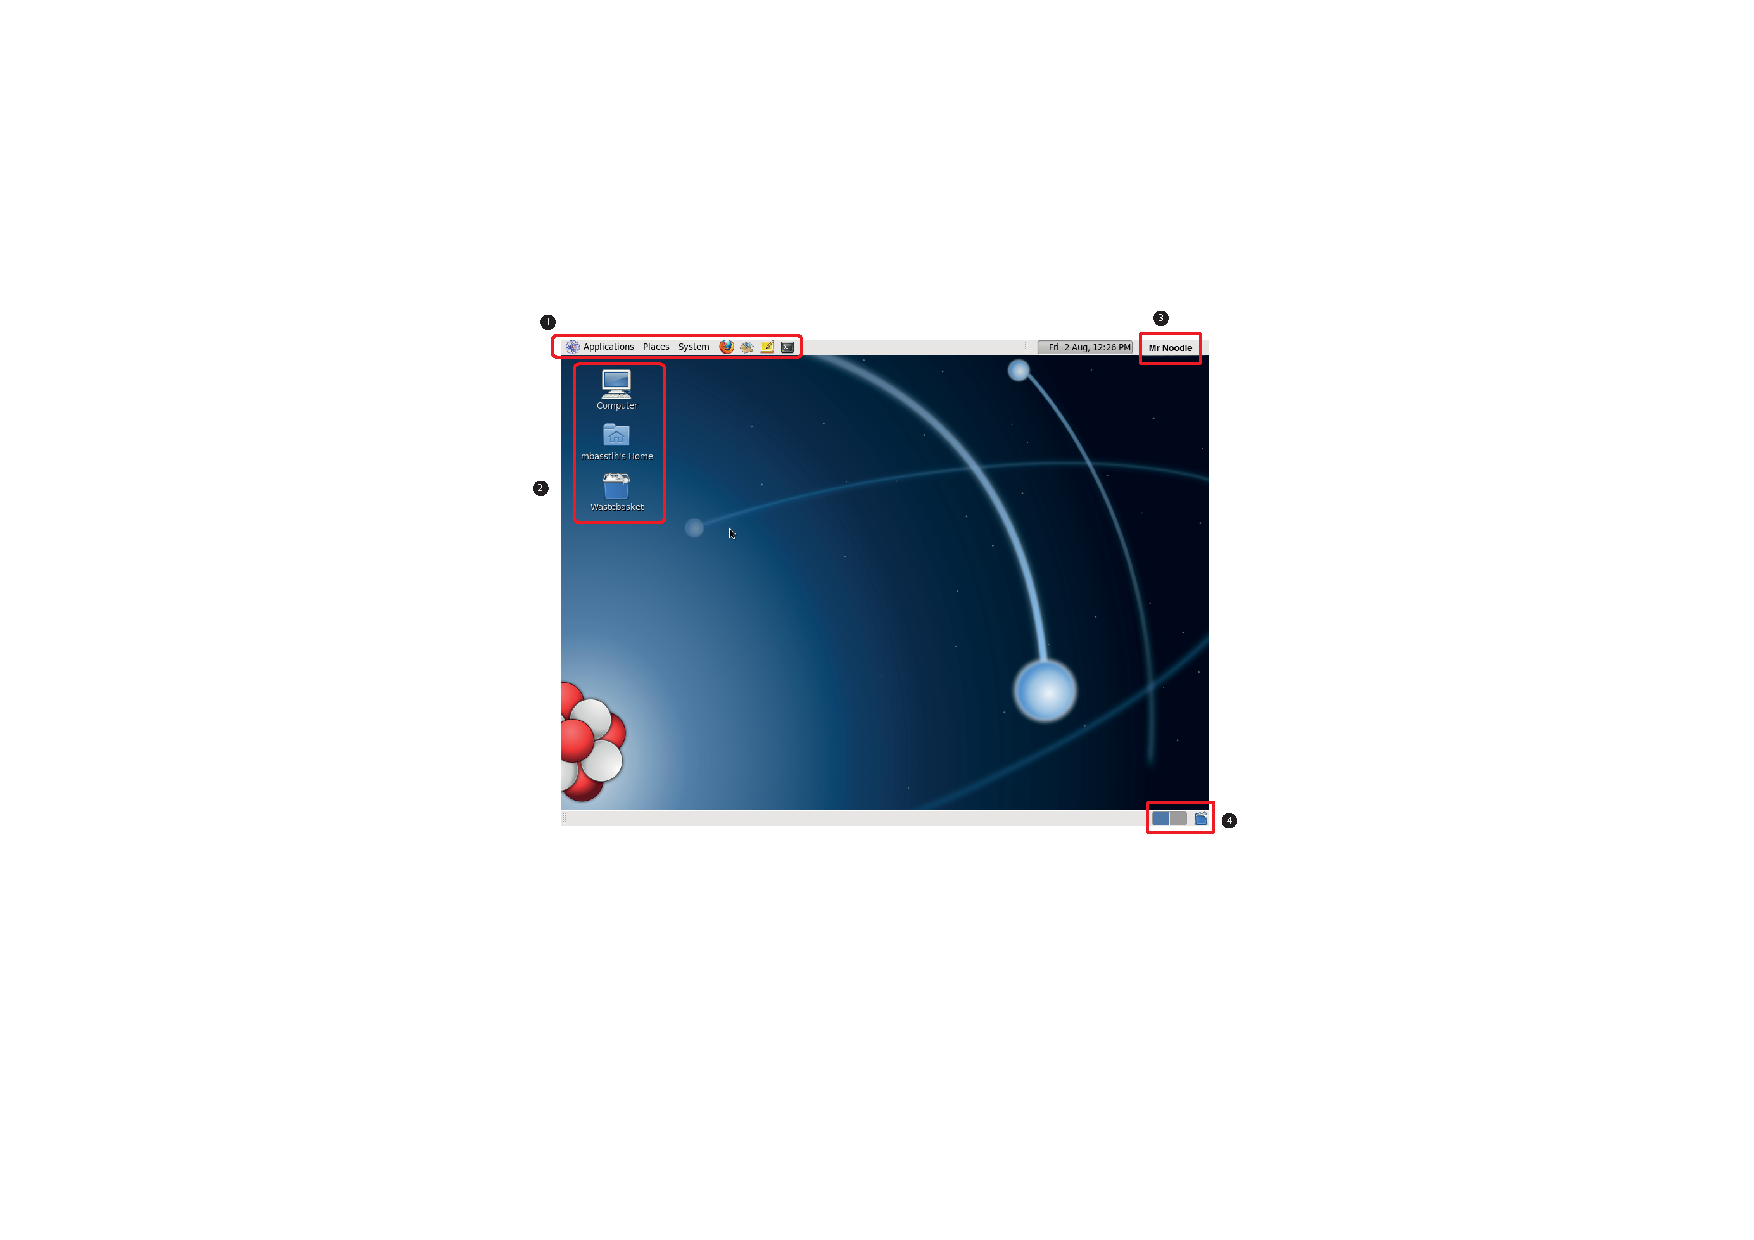
\includegraphics[width=16cm]{images/gnome-desktop}}
\caption{Scientific Linux's default graphical user interface and
  window manager, GNOME 2. \protect\circled{1} the top panel contains
  a menu of applications and system controls, as well as shortcuts to
  some frequently-used tools. You can easily configure the shortcuts
  to include your favourite things. \protect\circled{2} a graphical
  file-browser called `Nautilus' gives you graphical access to your
  files much like Explorer on Windows or Finder on
  OSX. \protect\circled{3} Clicking on your name shows the `log out'
  option. \protect\circled{4} The `wastebasket' and virtual desktop
  controls}\label{figure:gnome-desktop}
\end{figure}

Take a few minutes to explore the graphical environment. Even if you've never used Linux before, you'll probably find the general principles of this environment quite familiar: there are icons on the desktop giving you access to the computer via a graphical file browser, and at the top of the screen a menu-bar allows you to start various applications and utilities. The full manual for this environment---which is called GNOME 2---is available online at 

\noindent\urlnop{personal.us.es/rledesma/descargas/gnome2.6-user-guide.pdf}

\begin{linux}{GNOME and Metacity}
It's quite common to refer to GNOME as a `window manager', but technically it is much more than that; it's actually a collection of tools, applications and other programs that together form a graphical desktop environment. The window manager component of GNOME 2 is called \wikipedia{Metacity}{metacity}.
\end{linux} 

\noindent but you'll probably be able to work out everything you need to get you going by poking around at the various buttons. Unlike the Raspberry Pi where you have complete control over the operating system via the \texttt{sudo} command, the lab machines are configured so that you can't do any long-term damage to the setup. Apart from accidentally deleting your own files (and right now you have very little important stuff to accidentally delete!), there's nothing much you can do that will cause problems, so feel free to explore a bit. 

Perform the following tasks:
\begin{enumerate}
\item Find two different ways to start the Firefox web-browser.
\item Use Firefox to visit the School UG home page
  \urlnop{studentnet.cs.manchester.ac.uk/ugt/} and make this your
  home page in Firefox.
\item Work out how to change the desktop theme and choose one you like.
\item Create a keyboard shortcut for starting Firefox, to provide a third way of starting it.
\item Find the \wikipedia{Vector_graphics}{Vector Graphics} drawing application called Inkscape, and use it to draw a simple self-portrait. We just want you to spend a couple of minutes getting used to the kind of things that Inkscape can do---it will be very useful later in your degree programme when you're going to need to draw diagrams to go in your reports. For now any old doodle will do quite nicely (look at what Steve drew in Figure~\ref{figure:mrnoodle}, we're really not setting the bar very high at all here!) Make sure you save this file, we're going to need it later.
\item Figure out how to log out of the graphical environment. \label{list:logout}
\end{enumerate}

\begin{figure}[t]
\centerline{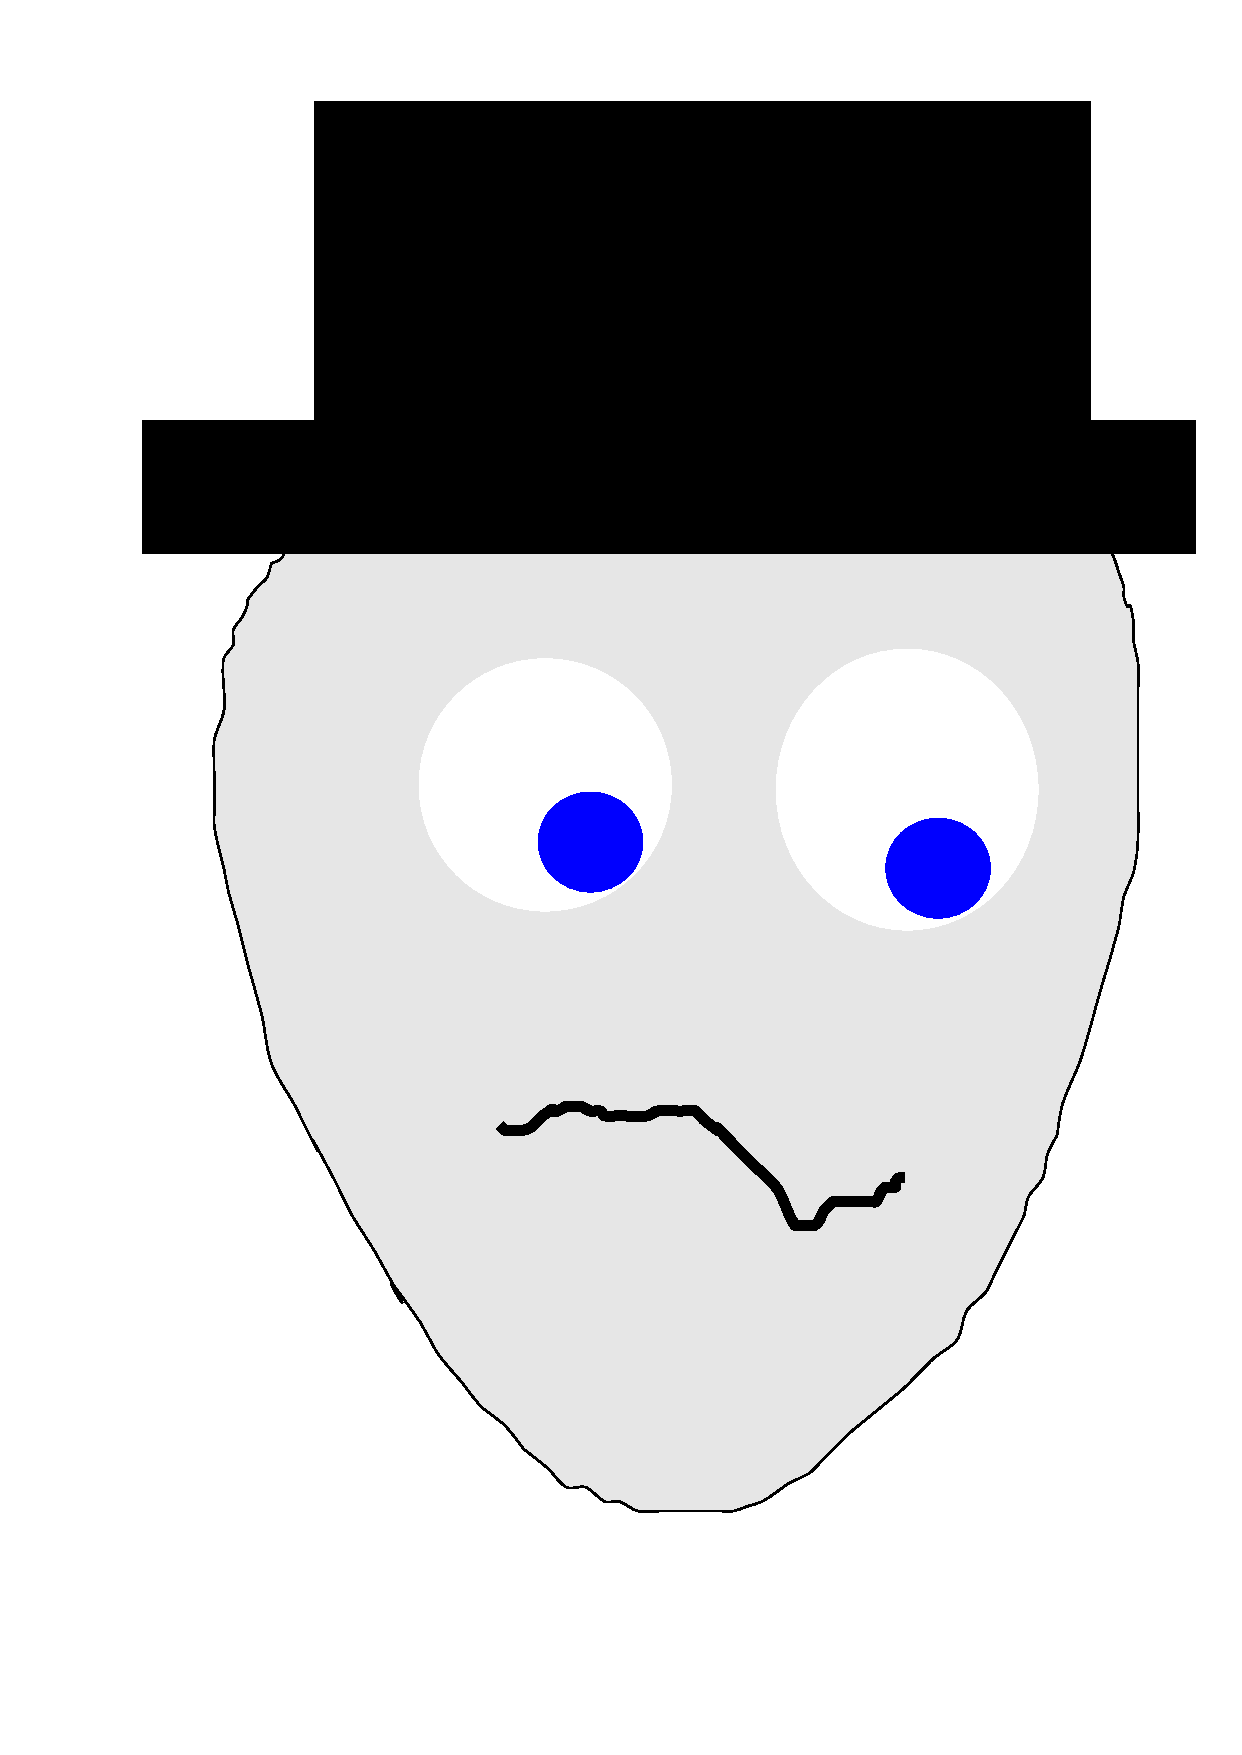
\includegraphics[width=0.25\textwidth]{images/mrnoodle}}
\caption{This is a picture of Mister Noodle drawn by Steve using Inkscape. It took about two minutes, though in reality had he spent any more time on it there would be no obvious improvement in the quality of the artwork.}\label{figure:mrnoodle}
\end{figure}

\begin{diversion}{Inkscape and GIMP: Vector and bitmap graphics}
Inkscape is a vector graphics drawing package; it allows you to draw and manipulate different shapes to create pictures and diagrams. It is ideal for drawing diagrams and figures. When you're using a tool such as Inkscape you're manipulating geometrical shapes such as points, lines and curves. One of the big advantages of this approach is that images look the same regardless of what magnification you use. In these notes we've tried where possible to use vector images, so you should be able to zoom into the pages on the electronic version without seeing any `pixellation' happening. Some figures contain a mixture of vector and bitmap graphics; for example, zoom into Figure \ref{figure:gnome-desktop} and you'll see that the image of the desktop itself starts to become jagged (because it's a bitmap), whereas the red boxes and numbers stay nice and crisp at any magnification (because they're vectors).

GIMP, on the other hand, is a bitmap based image manipulation package; it treats images as being made up of lots of coloured dots (pixels). GIMP is great for editing photographs and creating certain types of artwork, but it's not hugely useful for drawing diagrams. 

It's worth understanding the pros and cons of these two different approaches to graphics, it'll save you a lot of heartache later on and you'll end up creating more professional looking figures in your documents. The Wikipedia page on \wikipedia{Vector_graphics} provides a good explanation of the different approaches.

\end{diversion}

% \begin{note}
% Set up keyboard shortcuts?? Where should this go? Did one above for Terminal
% \end{note}

If you've completed step ~\ref{list:logout} you should now be back at the command prompt where you typed \cmnd{startx}{startx} a little while back. Before returning to the graphical environment where you'll spend most of your time, it's important to understand how the graphical interface you've just been using works as part of the Unix operating system. 

If you remember back to the first Raspberry Pi lab, we pointed out that the \texttt{shell} (\cmnd{bash}{bash}) that you're using to interpret commands is `just a program' that happens to interpret input from the user, execute commands, and display the results. The graphical environment you've just used is similar---just a program (or actually, collection of programs) that runs on the operating system.

But what do we mean by `execute commands'? You've probably got the hang of the fact by now that most of the things that happen in Unix are just programs stored somewhere on the file system (remember, you found some of them in the \texttt{/usr/bin} directory on the Pi). When you press Enter at a shell prompt, the  shell checks that what you've typed has a valid \concept{syntax}, and then starts up a new \concept{process} in which that program executes. The process is mostly independent of the shell program that started it, gets on with doing whatever it was designed to do, and when it finishes it tells the shell that it's done, and the shell gives you another prompt for the next instruction. Something very similar happens when you run the \texttt{startx} command: the graphical environment starts executing, and when you select the `log out' option, it returns you back to the shell so you can issue another command. Notice that you haven't been `logged out' of Linux, but rather just out of the graphical environment. 

Now, if you're going to use the graphical environment as your primary interface (and, as the jobs we ask you to do get more complex, you're going to need to!), you may find it slightly annoying to have to log into a lab machine, start the graphical environment, log out of the graphical environment when you're done \textit{and then remember to also log out of the console environment before you leave (because if you don't do this, other people will have access to your account!)}. 

Type the following:

\begin{ttoutenv}
\$ exec man ls
\end{ttoutenv}

You should find that the \texttt{man} command has done exactly what you normally would expect, but that instead of returning you to the command prompt when you exit, you've been unceremoniously logged out! Log back in again (sorry about that). 

The \texttt{exec} command changes the way in which the shell deals with whatever command follows it. Instead of starting a new process in which to run your command and waiting in the background for that command to complete, the shell gives up the process in which it itself is running, and hands it over to the command you've issued. So when that command finishes, there is no shell to come back to. And because in this case the shell was the first program that got run when you logged in, the Unix system logs you out since there's nothing else you can do. 

Experiment by running \cmnd{exec}{exec startx} and then logging out of the graphical environment as you did a moment ago; this time you should find that you've automatically been logged out of the console too.

But although that's one step closer to what we want, there's still the issue of having to type \texttt{exec startx} every time you log in. Of course this isn't a huge deal (it's certainly not as annoying as accidentally leaving yourself logged in at a console), but we can do better than this. 

When you first run the bash shell, it looks for a file in your home directory called \fname{.bash\_profile} and executes any commands it finds in there as though you'd typed them at the keyboard. Use the \cmnd{ls}{ls -a} command to confirm that there's already a file in your home directory called \fname{.bash\_profile}, and then use \cmnd{less}{less} to look at its contents. There should also now be one called \fname{.bash\_history}, take a look at it and it should become obvious how the \ttout{history} command, and the `reverse search' function you used earlier work.

\fname{.bash\_profile} should look something like this:

\begin{ttoutenv}
# .bash_profile

# Get the aliases and functions
if [ -f ~/.bashrc ]; then
	. ~/.bashrc
fi

# User specific environment and startup programs

PATH=$PATH:$HOME/bin

export PATH
\end{ttoutenv}

though don't worry if there are slight differences. We'll come back to what these instructions mean in a later lab. For now, start up the \cmnd{nano}{nano} editor, and use it to add a new line at the end of your \fname{.bash\_profile} that reads 

\begin{ttoutenv}
exec startx
\end{ttoutenv}

\textbf{It's really important that you don't put anything other than \ttout{exec startx} in your \fname{.bash\_profile}, so double-check you've got this right before moving on.}

Now log out (either type \texttt{logout} (or press \ctrl{d} to tell the shell that its input has ended), and log back in again. If all has gone to plan then you should see the graphical environment fire up automatically; and when you select `logout' from the menu, you should be returned to the Linux login prompt. 

Hurray!

\section{X Windows}

Let's take a step back now and look at what the \texttt{startx} command has actually done. Unlike OS X and Windows and most mobile operating systems, Linux doesn't really `have' a graphical windowing environment `built in'; what you've seen just now is a series of programs that co-operate with one another to  create the familiar WIMP environment.  If you don't know what WIMP means yet, go back and read Breakout~\ref{breakout:wimp} from the last lab session.

\begin{figure}[htb]
  \begin{center}
    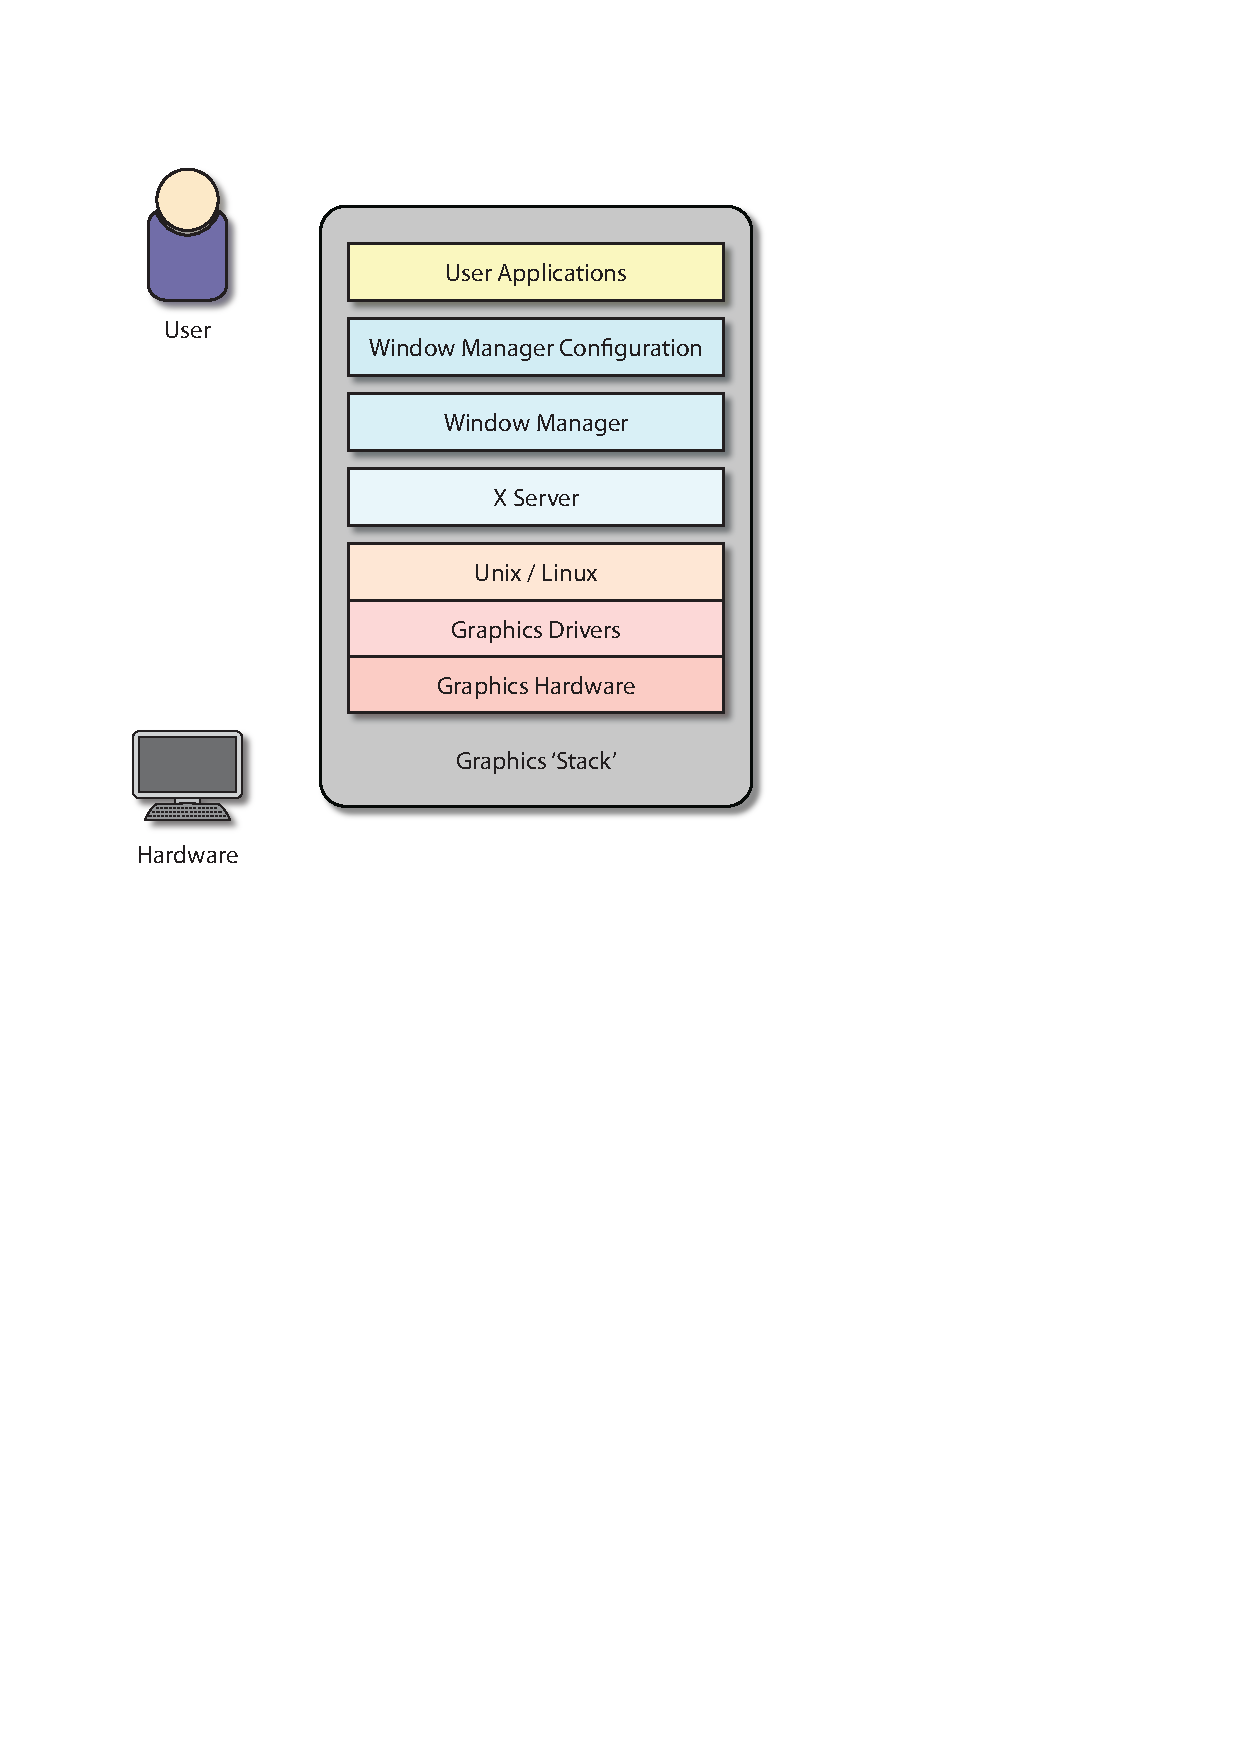
\includegraphics[width=.5\textwidth]{images/graphics-stack.pdf}
  \end{center}
\caption{The layered structure of Linux's graphical system, with software nearest to the underlying hardware at the bottom, and software closest to the user at the top.}
\label{figure:Xstructure}
\end{figure}

When you ran Quake and the snake game on the Pi in the previous lab, these programs took direct control of the graphics subsystem in order to display the game. The \texttt{startx} command runs a system called \wikipedia{X_Window_System}{X Windows}, which also communicates with the computer's graphics system, but on its own doesn't really do anything very exciting apart from allow other programs to then share the display. Along with X Windows, another system called a \wikipedia{Window_manager}{Window Manager} was started, and this is what you see drawing the buttons and menus and window controls for the graphical user interface. We'll look at how X Windows really works in one of the forthcoming \courseunit{COMP10120} lectures, and you'll explore the architecture of X Windows in a lot more detail in \courseunit{COMP18112} (Fundamentals of Distributed Systems) in the second semester. For now, it's enough to understand that there are two things going on here, first the X Windows system is running that allows stuff to be drawn to regions of the screen, and second the Window Manager which is doing all the WIMPy stuff like providing all the controls that allow windows to be moved and resized.

\begin{danger}{Killing X}
You can abort X Windows at any point by pressing Ctrl + Alt + Backspace on the keyboard, but this will abruptly kill the window manager as well as any other processes that you may be running, and is almost always a bad thing to do. Rather like removing the power from a computer without shutting it down properly, quitting X Windows in this way may cause you to lose data, or corrupt files, so should only use this as a last resort if more graceful ways of shutting things down have failed.
\end{danger}

\section{Terminal windows}
Your earlier use of the command line was on the computer's console, without X and a window manager running, but we now want to do similar things in GNOME. The tool to use here is a \concept{terminal window}. In GNOME you can fire up one of  these by clicking on the screen-like icon on the top panel.

% the \ttout{Applications} menu at the top of the screen, then \ttout{System Tools}, then \ttout{Terminal}.

Most of what you do in these and future labs will involve using terminal windows in one way or another.

% It's a good idea to give yourself easy access to a terminal window by right clicking on the Terminal menu item and selecting \ttout{Add this launcher to panel}. You will then see a terminal icon on the top panel which you can use to start a terminal window whenever you wish to.


\section{The Awesome Window Manager} 
One of the interesting effects of the X architecture, shown in Figure~\ref{figure:Xstructure}, is that you can use different window managers on Linux, and can choose the one that best suits the way you work; some people like `rich' environments like GNOME, whereas others like `lean' cut-down window managers. 

To demonstrate this, start a terminal, and use \cmnd{nano}{nano} to create a file in your home directory called \fname{.Xclients} (don't miss the leading \ttout{.} in the file name), and in that file put a single line that reads:

\begin{ttoutenv} 
exec awesome
\end{ttoutenv}
 
The file \fname{.Xclients} is \concept{executed} as part of the process of starting the X windows system, so we need to do one more thing to  enable this. Use the following command:
\begin{ttoutenv}
chmod +x .Xclients
\end{ttoutenv}
We'll explain more about \cmnd{chmod}{chmod} and \concept{file permissions} in the next lab session.

Now quit GNOME, and log back in; this time, instead of GNOME (which is set to be the default desktop in the case where you've not told the system otherwise by creating a \fname{.Xclients} file), you should be given the Awesome window manager.

Awesome is a very minimalist window manager, probably quite unlike anything you've used before. Most WIMP environments that you'll have used so far make you the user responsible for the position and size/shape of the windows that represent tools and applications on the desktop. The upside of this is that you can arrange things exactly as you like them; the downside is that you probably use up an amount of time doing that arrangement, and often end up with a layout that wastes some of the desktop's usable space. Awesome is what's called a `tiling' window manager; instead of giving you detailed control over the exact shape of windows, it lays them out on the screen in one of several configurations designed to maximise the use of space. Because you can't drag or resize windows with the mouse, there's no need for the usual window decorations, so you save a few pixels this way too. To create a window, use the icon in the top-left of the Awesome desktop. Make a few terminal windows, and then cycle through the different layouts available using the icon in the top right. 

There's no doubt that Awesome is at the hard-core end of the window manager spectrum, and its designed for experienced users that needs very large numbers of windows open at once, probably spread over several physical displays (as in Figure \ref{figure:awesome}). Apart from the `tiling' aspect, it gives you virtually no visual cues as to how to perform various actions, most of which are designed to be invoked via keyboard shortcuts (in fact, Awesome is designed so that you can use all of its features without needing to touch the mouse at all.) Once you've remembered all the keyboard combinations, using a window manager like Awesome can be extremely efficient in terms of time and screen-space, but you may find using this at the same time as learning your way around Unix a bit daunting right now, so feel free to swap back to using the rather more friendly environment provided by GNOME. To do this, use one of the terminals to rename the \fname{.Xclients} file you created a moment ago (the command \cmnd{mv}{mv .Xclients  .Xclients.awesome} will do this), and quit Awesome using the option available via the top-left menu. Log back in again, and you should have GNOME once more. 

\begin{figure}[htb]
  \begin{center}
    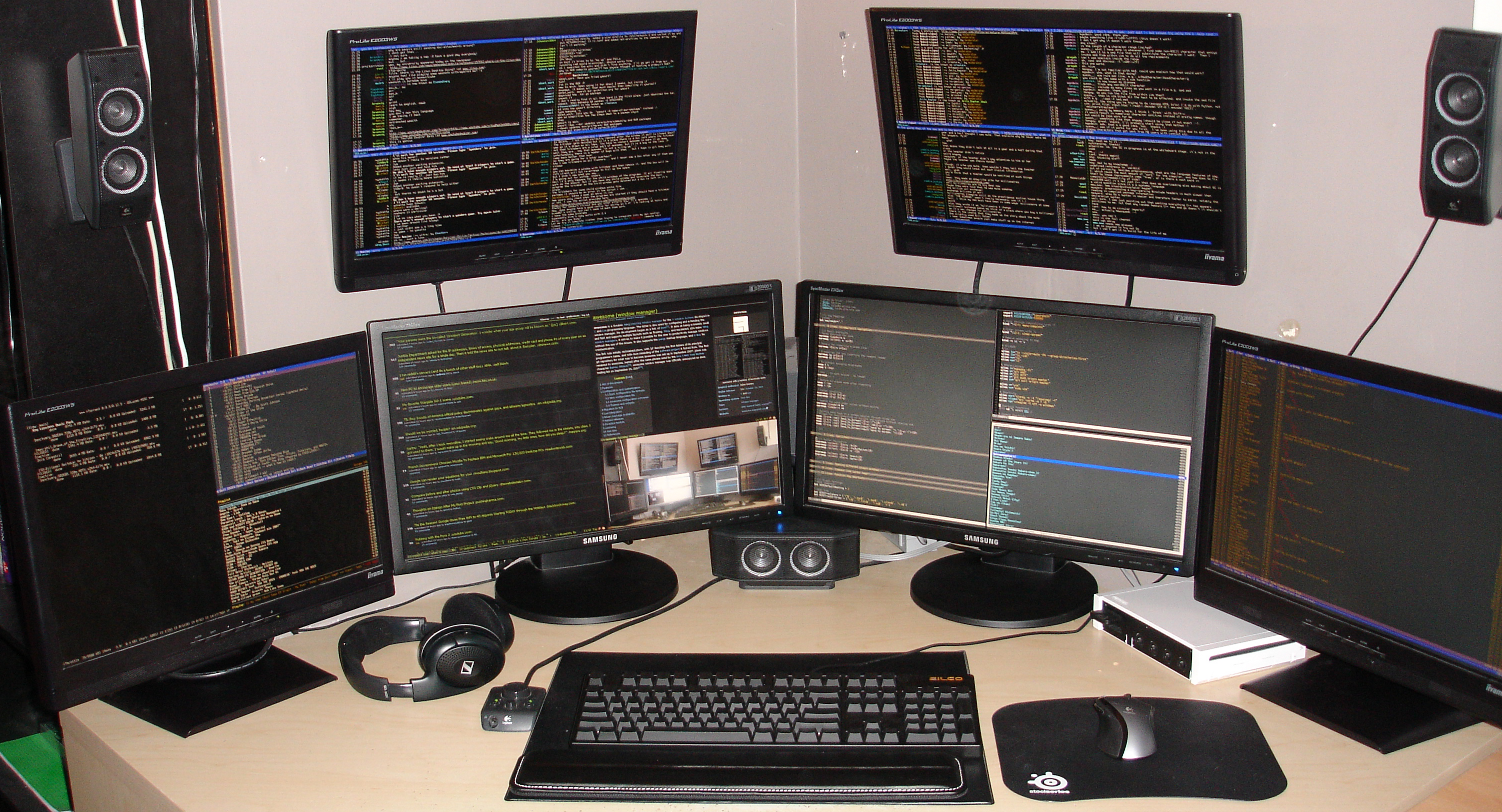
\includegraphics[width=14cm]{images/awesome.png}
  \end{center}
\caption{The Awesome window manager showing around 20 windows tiled over 6 physical displays. Reproduced from \urlnop{awesome.naquadah.org} with kind permission of Julien Danjou, one of Awesome's primary authors.}
\label{figure:awesome}
\end{figure}

As you become more familiar with Unix principles, keep the fact that you can easily swap window managers in mind. Most likely there will come a point where the graphical niceties of environments like GNOME become unnecessary, and perhaps even a distraction from getting work done, and you might find that a slimmed down window manager suits you better as a more experienced `power user'. For the rest of these exercises, though, we'll assume you're using GNOME (if you're confident enough to use something else, then translating our instructions to make sense in whatever environment you've chosen won't be too big a problem). 

% \begin{note}
% Could be link to JTL's ALU tutorial here. If it exists
% \end{note}


% \begin{note}
% Where does backgrounding and nohuping go? desktop2
% \end{note}

% \begin{note}
% What about virtual consoles? This could be a link to JTL's extended tutorial. If it exists
% \end{note}

% \begin{note}
% Test out which other WMs are installed; can you kill X server from the keyboard?
% \end{note}

%\printbibliography

\FloatBarrier

\section{ARCADE}

We would now like you to register your access to the ARCADE server. ARCADE is the laboratory management system we use to administer coursework marks and deadlines, etc.. You can use the client query program to look up your details, laboratory timetables, marks, and so on, throughout the year. It is recommended you do this fairly regularly, if only to check that mistakes have not been made in your marks! You need to register with ARCADE before any of your lab work can be submitted, so it is much better to do it now than wait until your first deadline!

In a terminal window, run the command \ttout{/opt/teaching/bin/arcade}; after a short pause, a new window will pop up. In the large text box you should find a message telling you that you are not yet authenticated, and that you have just been sent an email. If this is so, then quit the program, read the email you have just been sent by the ARCADE server, and carefully follow the instructions in it. Then you will start the ARCADE Query client again, and it should now connect you to the server. If this works, then your access is set up!

Explore the various queries of the client, and familiarise yourself with the the user interface. Check that your registration details are correct. Feel free to ask for explanation if it is not obvious to you.

\section{Text Editors}

% \begin{note}
%   Need something for them to do here with editor. Idea was to fix .bash profile to prevent the problem when using ssh. But ssh not introduced until the next lab!

%   Now fixing PATH

%   Minimal change seems to be

% \begin{alltt}
% case `tty` in
% /dev/tty*) exec startx
% esac
% \end{alltt}
% \end{note}

A great deal of the lab work you will be doing over your time here
will involve you creating text files of various kinds, often source
files in a programming language such as \ttout{Java}, \ttout{PHP} or
\ttout{C}, or \ttout{HTML} files for use on the web. There are
specialist tools called
\wikipedia{Integrated_development_environment}{Integrated Development
  Environments} or \emph{IDE}s that can be used for programming; you
will meet these later in your programme. However, for many purposes,
the simplest, and best, tool for creating such files is a simple text
editor. You have already met one such tool, \ttout{nano}, which is
fine for work at the console or quick modifications of existing files,
but for more extensive work an editor that takes advantage of X's
graphical capabilities is more appropriate.

The Linux environment in which you will be working offers many such
editors, including the default GNOME editor \ttout{gedit}, the KDE
editor \ttout{kate} and the grand daddy of all editors,
\ttout{emacs}. These three are illustrated in Figures \ref{fig:gedit}
and \ref{fig:texteditors}. They are all shown ready to edit a
\ttout{Java} source file; note that they all use the fact that this is
\ttout{Java} source to highlight key words within the text. When you
have some free time, please do experiment with some of the text
editors available and find one that you like; in the meantime you
should probably use \ttout{gedit}.

\begin{figure}
  \centering
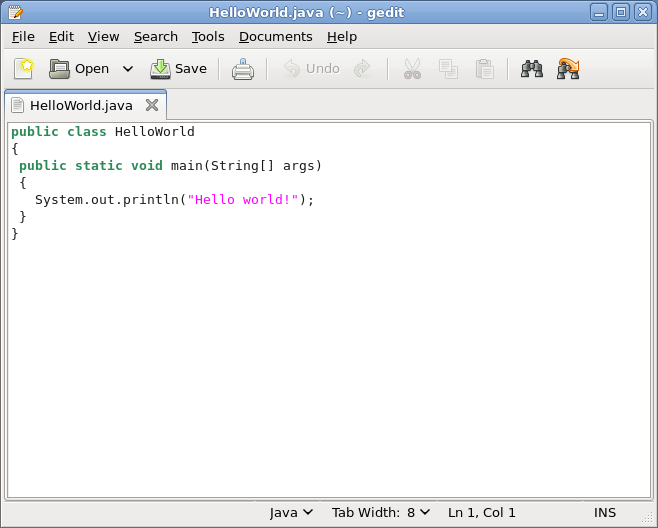
\includegraphics[width=.7\textwidth]{images/gedit}  
  \caption{\ttout{gedit}}
  \label{fig:gedit}
\end{figure}

\begin{figure}
  \begin{minipage}[b]{.5\linewidth}
    \centering
    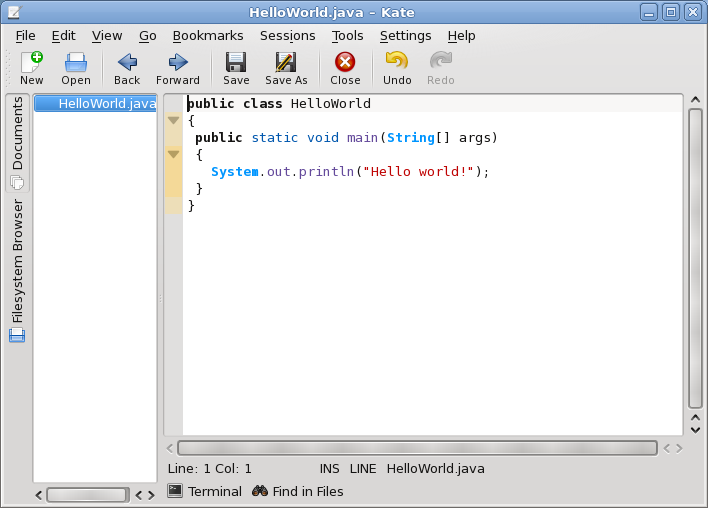
\includegraphics[width=.8\textwidth]{images/kate}  
    \subcaption{\ttout{kate}}\label{subfig:kate}
  \end{minipage}%
  \begin{minipage}[b]{.5\linewidth}
    \centering
    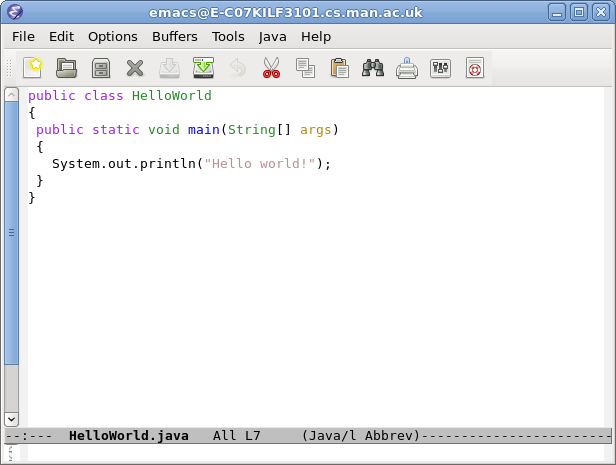
\includegraphics[width=.8\textwidth]{images/emacs}
    \subcaption{\ttout{emacs}}\label{subfig:emacs}
  \end{minipage}%
  \caption{Other editors}  \label{fig:texteditors}
  
\end{figure}

\section{Shell environment variables}

When you started the ARCADE client earlier, you had to type its full
pathname, which is \fname{/opt/teaching/bin/arcade}. The directory
\fname{/opt/teaching/bin} is a place where we keep lots of useful
teaching related tools, so it would be useful if you didn't have to
type it every time you want to use a program from there; luckily
there's a way of doing this. When you type a command on the command
line, the shell looks for a program of that name in a number of
places. These places are determined by the value of a shell
\wikipedia{Environment_variable}{environment variable} called
\ttout{PATH}. You can see what its current value is by using the
command

\begin{ttoutenv}
\$ echo \$PATH
\end{ttoutenv}

This will show a long list of directories, separated by colons (\ttout{:}).

There are many other shell variables already set for you, they can be
seen by running the shell command \cmnd{set}{set} (do this now). How do you stop the
output scrolling off the screen? Most of these variables won't make
much sense to you at the moment, but among them are \ttout{HOME},
\ttout{PWD} and \ttout{HOSTNAME}; you can check their values using
\cmnd{echo}{echo}. What do think their values represent?

You can set the value of a shell variable at the command line, for example:

\begin{ttoutenv}
\$ MYVAR=42
\$ echo \$MYVAR
\end{ttoutenv}


Note that they should be no spaces either side of the \ttout{=} sign and that the variable's name is \ttout{MYVAR} and its value is obtained  by using \verb+$MYVAR+. If a variable is given a value on the command line in a terminal window like this its value is only available in the shell running in that window.

In order to be able to start the ARCADE client by typing \ttout{arcade} rather than the full pathname \ttout{/opt/teaching/bin/arcade} we need to modify the \ttout{PATH} variable to include the directory \fname{/opt/teaching/bin}. We can do this on the command line by typing

\begin{ttoutenv}
\$ PATH=\$PATH:/opt/teaching/bin
\end{ttoutenv}

This can be read (and you will see this over and over again in
programming languages) as 'find the value of the right hand side of
the \ttout{=} and give (or \concept{assign}) that value to the variable on the left hand side'. So this takes the current value of \ttout{PATH} and adds
\ttout{:/opt/teaching/bin} on the end. After you've done this you can
type \ttout{arcade} in your terminal window and the ARCADE client
should start. Just exit it cleanly and return to the shell.

% \begin{note}
%   Background jobs? Where do these go? desktop2? Yes.
% \end{note}

If you now start another terminal window and type \ttout{arcade}, what happens and why?

The way to make the change permanent is to modify your
\fname{.bash\_profile} file. While we are doing this we will also add
another useful directory to our PATH, namely \fname{/opt/common/bin},
another shared directory containing useful stuff.

Use \ttout{gedit} to modify  \fname{.bash\_profile} by adding the following line \emph{immediately before the existing line starting with \ttout{PATH}}.

\begin{ttoutenv}
PATH=\$PATH:/opt/teaching/bin:/opt/common/bin
\end{ttoutenv}


This won't have any effect until you logout and login again. So do that now and try starting \ttout{arcade}. Run \ttout{echo \$PATH} and you will see the new value, with your own \ttout{bin} directory at the end, preceded by the two \ttout{/opt} directories.

Before we move on to mail reading, we would like you to make another modification to your \fname{.bash\_profile} file. Earlier you added the line \ttout{exec startx} to fire up X automatically when you login. This works fine when you login directly to a PC, but will cause problems if you login remotely from another machine, as you will in the next lab. We won't explain the exact meaning of this piece of code now but will do in a later lab.

Replace the line \ttout{exec startx} at the end of \fname{.bash\_profile} with the lines

\begin{ttoutenv}
case `tty` in
/dev/tty*) exec startx
esac 
\end{ttoutenv}

\emph{Note that the characters surrounding \ttout{tty} are back-quotes, not forward quotes. This character can be found on the keyboard of lab machines in the top left hand corner, just below \ttout{Esc}.}

You should now logout and login again to check that GNOME has started, which means that this has worked. We now move onto configuring a mail client for you to use.

\section{Configuring Thunderbird}

% \begin{note}
% These instructions need changing in the light of Hamza's experience.  
% \end{note}

Rather than explain the Thunderbird configuration here we refer you to an illustrated guide to this process, which you can find at \url{http://wiki.manchester.ac.uk/compsci/index.php/How_to_set_up_Office_365_Mail_in_Thunderbird}, written by a fellow student.

Follow all three steps in the process described in this document.

% Follow these steps and refer to Figure \ref{figure:thunderbird} to configure Thunderbird to read your University email. Start the Thunderbird application (you'll find it in GNOME's Applications menu, and might want to create a keyboard shortcut for it, as well as dragging and dropping the icon up on the top panel for easy access next time). 
% \begin{enumerate}
% \item The first time you run Thunderbird, it will ask you to create an account as shown in panel (a). Click the `Skip this and use my existing email' button. 
% \item In dialogue (b) enter your full name (not a nickname), your email address (which will be something like firstname.lastname@student.manchester.ac.uk), and your University password in the appropriate fields. 
% \item Press `Continue', and wait a bit while Thunderbird tries (and fails!) to guess the rest of the settings for you (there's no guessable relationship between your 8-character username and your email address really, so its not hugely surprising that Thunderbird can't figure out the settings automatically). 
% \item When the dialogue window shown in (c) appears you will need to correct some of the settings that Thunderbird has tried to guess. First change the contents of the \ttout{Username} box to your proper username, then change the server settings. The correct values for these are:\\
% \\
% {\small
% \begin{tabular}{llllll}
%  & & \textbf{Server Hostname} & \textbf{Port} & \textbf{SSL} & \textbf{Authentication} \\
%  \\
% \textbf{Incoming} & IMAP & email.manchester.ac.uk & 143 & STARTTLS & Normal password\\

% \textbf{Outgoing} & SMTP & outgoing.manchester.ac.uk & 587 & STARTTLS & Normal password
% \end{tabular}
% }
% \item If you've entered these correctly, press `Done', and you should be able to send and receive email (if you accidentally press `Re-test' at this stage, Thunderbird will once again fail to guess the settings, and you'll need make a change and then unmake that change in any of the text fields in order for the `Done' button to become active again).

% \item Before you use Thunderbird to read your mail, you should make one more change. Thunderbird's default behaviour is to make a local copy, or \concept{cache}, of all your email messages in your home filestore. In many circumstances this is a very useful thing to do, but with our student setup can cause problems by unnecessarily using up some of your filestore quota. To turn this behaviour off follow these steps:
%   \begin{itemize}
% \item Click on the account name in Thunderbird's left hand panel
% \item Select \ttout{View settings for this account}, then \ttout{Synchronisation and Storage}
% \item Untick the box \ttout{Keep messages  for this account on this computer.}
%   \end{itemize}
% \end{enumerate}


%\begin{note}
% Looks like the last point in the previous points is in small! SRP can't see what the problem is. Fixed, it was SRP's mistake!
% \end{note}

% \begin{note}
% REMEMBER WE MUST FIND OUT HOW TO DISABLE DOWNLOAD/CACHING OF EMAILS


% \end{note}

% \begin{note}
%   Might be worth making the figure into 3 or 4 separate things to allow them to be bigger.

%   email address should be @student.manchester....
  
% \end{note}

% \begin{figure}[h]
% \centerline{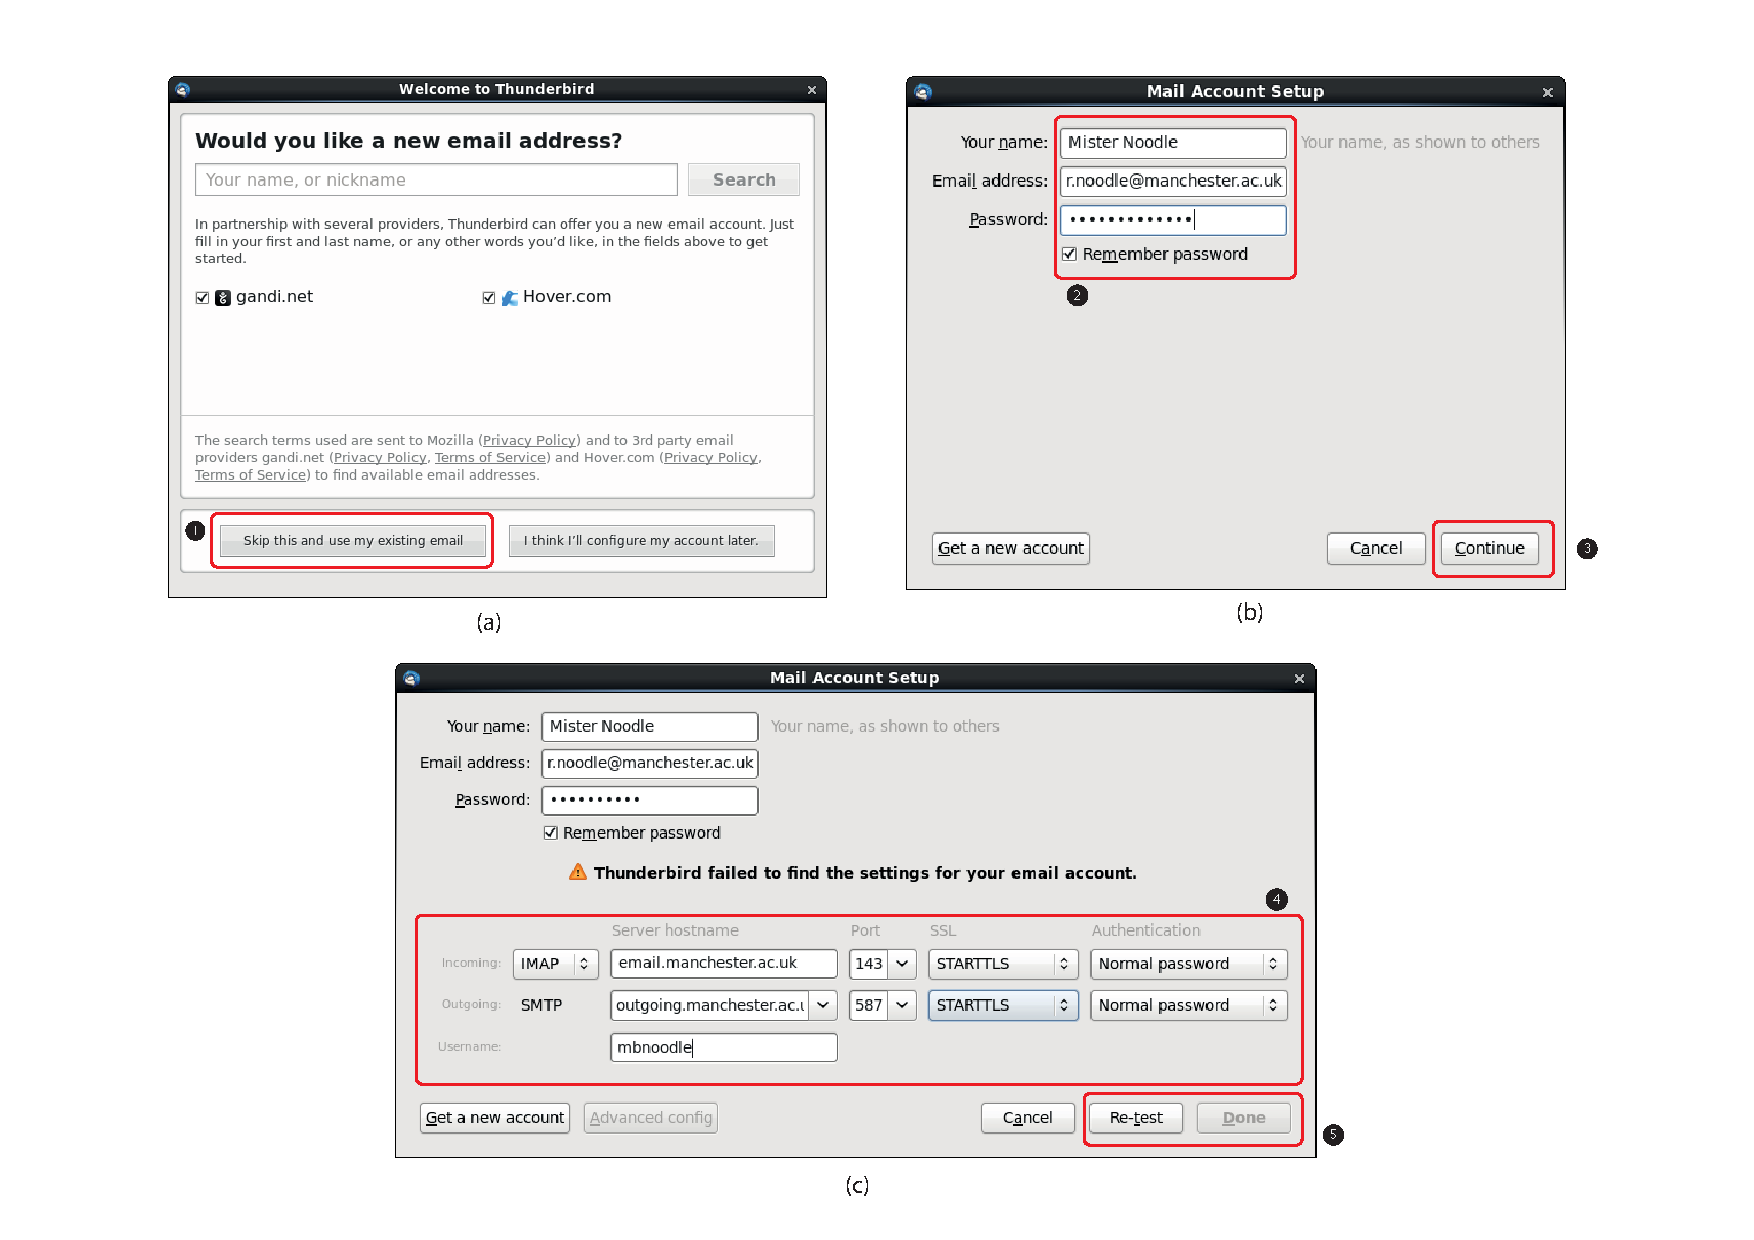
\includegraphics[width=17cm]{images/thunderbird-instructions}}
% \caption{}\label{figure:thunderbird}
% \end{figure}

Once your Inbox appears in Thunderbird, using it to compose and send email should be fairly self-explanatory, but if you're stuck there are plenty of Thunderbird tutorials available on the web. 

\section{That's all for now}
\label{sec:thats-all-now}

If you have reached this point before the end of the lab you may have gone too fast so please go back and review what you have done. You will be using many of the ideas we've just met in later labs, so it's important to understand them.


% \section{Exploring the CS Unix environment -- which RPMs are installed}

% \begin{note}
%   Do we need this? Could it go in desktop2?
% \end{note}



